\documentclass[10pt,a4paper]{article}
\usepackage{amssymb, amsmath, amsbsy} % simbolitos
\usepackage{multirow}
\usepackage[spanish,es-tabla]{babel}
\usepackage[utf8]{inputenc}
\usepackage[spanish]{babel}
\usepackage{amsmath}
\usepackage{amsfonts}
\usepackage{amssymb}
\usepackage{graphicx}
\usepackage{multicol}
\usepackage{titling}
\usepackage{titlesec}
\usepackage{array}
\usepackage{bm}
\usepackage{afterpage}
\usepackage{float}
\usepackage{graphicx}
\usepackage{epstopdf}
\usepackage{longtable}
\usepackage{epigraph}
\setlength\epigraphwidth{1.5\textwidth}
\usepackage{subfigure}
\usepackage{anyfontsize}
\graphicspath{{informe 2/}}
\usepackage[left=2cm,right=2cm,top=2cm,bottom=2cm]{geometry}
\usepackage[colorlinks=true,
            linkcolor=blue,
            citecolor=blue,
            urlcolor=blue]{hyperref}
                     
\begin{document}
\author{Kevin A. Enriquez-Fuel, Kevin G. Oñate-Pozo, Fredy D. Chicaiza-Chuquilla}
\title{Universidad Tecnica Del Norte\\ Fica-Ciercom\\ Sistemas Embebidos\\Examen Bimestral I \\}
\maketitle
\begin{multicols}{2}
\begin{itemize}
\section{Objetivos}
\item[•] Realizar una revisión bibliográfica sobre el funcionamiente de los sensores: MQ-7, MQ-135, Sensor de Rayos UV ML8511, Sensor de temperatura TH y el microprocesador MCU.
\item[•] Calibrar los sensores para obtener datos precisos
\item[•] Documentar el funcionamiento y parámetros de los sensores.
\item[•] Realizar el armado de la placa.
\section{Introducción}
\subsection{Primera Lectura: Calidad del aire y efectos en la salud-¿Como pueden contribuir las redes de sensores inalámbricas?}

Uno de los principales problemas que afectan a todos
los países, no solo en aquellos que están dentro de
grandes metrópolis o en zonas industriales: La contaminación
 del aire, es un gran problema que desemboca
grandes daños, riesgos a la salud y un fuerte prejuicio
económico para todas las naciones del mundo.
El principal objetivo de este artículo, es plantear
diferentes alternativas para brindar una posible solución
 frente a este problema. Con la introducción de la
tecnología y las capacidades de la Internet de los objetos
(IO) se pretender disparar nuevos casos de uso y
aplicarla a diferentes entornos.

Para el análisis de los parámetros anteriormente
nombrados, se utilizaran los sensores: Quimioluminiscencia,
difusión pasiva (DP) y Los sensores electroquímicos.

\subsubsection{Detectores de quimioluminiscencia}
El principio de medición se basa en sobre la reacción radiactiva
del ozono con el óxido de nitrógeno (NO).
Esta radiación puede ser detectada para medir la
cantidad de NO. El NO2 puede medirse separando
el NO2 para obtener el NO por medio de los
rayos UV.

\subsubsection{Muestreadores de difusión pasiva}
Es un método
de medición integral, es decir, mide todo el NO2
desde el momento en que fue montado, hasta la
hora en que se recoge.


\subsubsection{Sensores electroquímicos}
Los sensores electroquímicos consisten ende al menos dos electrodos.
El gas se difunde en una cámara, que normalmente
está cubierta por una membrana, para
proteger de partículas que entran en la cámara.



\subsubsection{Sensores Ópticos}
Los sensores ópticos se basan
en la absorción de luz por gases. Del ultravioleta
al infrarrojo, cada molécula tiene un espectro
de absorción específico.

\subsection{Segunda Lectura: Impacto de las emisiones de NOx en el clima y la monitorización mediante la tecnología de sensores inteligentes}

En este articulo se intento diseñar un sistema de
Flame monitoring, pero con un sistema muy simple de
procesamiento de imágenes para controlar las emisiones
de CO. Por lo tanto, la investigación en este campo
encuentran muchas posibilidades que permitirán a los
investigadores desarrollar una técnica aborigen para el
sistema de ame monitoring.
Brown et al (2008)desarrollo un chip de fotodiodo
de carburo de silicio doble para determinar la temperatura
de un producto natural. El concepto que aquí se
discute utiliza el cambio en la forma de la banda OH
(260-350 nm) con temperatura. La mitad del chip estaba
cubierta con un filtro dieléctrico de capas múltiples
con una longitud de onda corta de alrededor de 315 nm.
Despues de la amplificación, las dos señales produjeron
por las partes filtradas y no filtradas de la viruta, que
se dividen para producir una proporción, que es muy
sensible a los cambios en la temperatura de la llama. La
sensibilidad es de aproximadamente 0.35en la temperatura
de la llama para temperaturas entre 2700 y 3000
grados Farenheit. La temperatura medida es la medida
especifica temperatura comprendida por el campo de
visión del sensor.
El objetivo es desarrollar sensores de avance para
reducir el NO, emisiones de CO y CO2 que mejoran
la combustión efectiva. En este método propuesto por
Ronald Hanson et al. (2004), un laser de diodo de infrarrojo
cercano sintonizable y de absorción se utiliza
la espectroscopia. Estrategias de control para la combustión
, implica una temperatura del gas robusta y de
respuesta rápida sensor, sensor de fibra acoplado para
la temperatura del gas, O2, CO y una nueva técnica
para la detección de hidrocarburos no quemados.

\subsection{Tercer Lectura: Polluino: una gestión eciente basada en la nube de Dispositivos IoT para monitoreo de calidad del aire}

La idea fundamental del Internet de las cosas es la
distribución de los objetos ``ubicuos o cosa", que recogen
e intercambiar datos con el fin de alcanzar un objetivo
común a través de interacciones mutuas [1].Polluino,
es un dispositivo de sensor basado en Arduino
que recoge y transmite los datos recogidos por múltiples
módulos de sensor. En detalle, los parámetros ambientales
se recogen con el objetivo de medir los niveles
de contaminación del aire. El encendido / apagado de
conmutación de los sensores se controla a distancia de
acuerdo a los datos basados en sensores que se almacenan
y administran directamente en la infraestructura
de Cloud. El Arduino recoge todos los datos de los sensores
y los envía a la plataforma en la nube mediante
el uso de la ESP8266 modulo Wi-Fi, que está conectado
al Arduino a través de un puerto serial de a bordo.
Ciudad inteligente guion. Las características típicas de
Ciudades inteligentes son la movilidad y la variedad
de nodos (dispositivos móviles de usuario, sensores, y
vehículos), que puede ser equipado con al menos una
interfaz de red, y la amplia disponibilidad de puntos
de acceso inalámbrico.
El enfoque propuesto podrá utilizarse para hallar una
manera  optima de controlar luces trafico c, a  fin de mejorar
trafico c minimizando al mismo tiempo los niveles
de contaminación de aire. Por otra parte, este trabajo
futuro se centrara en la comparación entre los protocolos
MQTT y COAP.

\subsection{Cuarta Lectura: Desarrollo de plataforma de detección para mediciones y análisis de calidad del aire}

AAB College, han desarrollado e implementado una
plataforma de detección en el laboratorio, que mide la
calidad del aire, que puede ser utilizado para monitorear
y puede proporcionar datos para su análisis. Esta
plataforma se basa principalmente en la tecnología  Arduino.
Se han calculado y el valor AQIs de diferentes
contaminante, tales como SPM (partículas suspendidas),
NRMF (respirable partículas suspendidas), SO2,
NO2, etc, en la India, Delhi. Monitorearon tres sitios
diferentes. Recibieron muestras dos veces por semana,
por lo que durante un año se recogieron 104 muestras.
Las muestras recogidas se analizaron mediante diferentes
métodos prescritos por APHA1977 (American Public
Health Asociación). Los sensores electroquímicos
son los tipos más rápido crecimiento, para este proyecto
se ha utilizado sensor Shiney PPD42, que se utiliza
para el cálculo de la calidad del aire, principalmente
para la concentración de PM10 en burbujas de polvo,
pero también es compatible con las mediciones de PM.
El Índice de Calidad del Aire (AQI) es muy importante
con el fin de identificar la calidad del aire en ambientes
diferentes. Hay diferentes sistemas que pueden calcular
el índice AQI. Estos sistemas deben ser capaces de
monitorizar diferentes contaminantes del aire en tiempo
real, informando a la gente sobre el estado actual
de la calidad del aire y el envió de la información a un
servidor centralizado, que a su vez puede generar estadísticas e informes. Se ha desarrollado un algoritmo
llamado ``Algoritmo para el cálculo del índice". El objetivo
de este algoritmo es calcular la calidad del aire,
sobre la base de los valores tomados de AQI estándares
(Índice de Calidad del Aire), y para mostrar resultados
en formato básico en la pantalla LCD y (pero no
limitados a) muestran el color correspondiente o combinación
 de colores de las luces LED.

\subsection{Quinta Lectura: Sistema de monitoreo de la contaminación del aire urbano con modelos de pronostico}
Se cree ampliamente que la contaminación del aire
urbano tiene un impacto directo en la salud humana,
especialmente en los países en desarrollo e industriales,
donde las medidas de calidad del aire no están disponibles
o se implementan o aplican de manera mínima.
Se presenta una red basada en sensores inteligentes que
se comunican mediante una red de área local inalámbrica
para aplicaciones de monitoreo de la calidad del aire.
Esta red utiliza redes neuronales artificiales (ANN)
para estudiar los efectos de la temperatura y la humedad
en las concentraciones de contaminantes. Principalmente
se centra en presentar un NGAM piloto y
en el desarrollo de modelos de pronostico precisos para
predecir las concentraciones promedio futuras de algunos
contaminantes del aire urbano, a saber: O3, NO2 y
SO2, todos los cuales se mencionan como perjudiciales
en Las directrices de la OMS.
La calidad del aire es un problema importante que afecta
directamente la salud humana. Los datos de calidad
del aire se recopilan de forma inalámbrica a partir de
motos de monitoreo que están equipados con una variedad
de sensores gaseosos y meteorológicos. Estos datos
se analizan y utilizan para pronosticar valores de concentración
de contaminantes utilizando una plataforma
inteligente de maquina a máquina. La plataforma utiliza
algoritmos basados en ML para construir los modelos
de pronostico aprendiendo de los datos recopilados.
Estos modelos predicen 1, 8, 12 y 24 horas antes de los
valores de concentración.



\section{Marco Teórico}
\subsection{Filtro Medio}
El filtro medio es uno de los métodos de suavizado más simples. La versión modificada de este algoritmo se discute en [1], [2]. El valor de salida se calcula calculando el promedio de todas las muestras de la ventana. Su fórmula tiene la siguiente forma:

\begin{equation}
z_{j} = \frac{\sum_{i=-n}^n  x_{j+i}}{2n+1},
\end{equation}

donde $xi$ es una muestra de la señal de entrada, $2n + 1$ es la longitud de la ventana, $zj$ representa el valor de salida y j es el índice actual del valor de salida. Se conocen diversas formas de promediación. Uno de ellos es el uso de la máscara de filtro que consiste en números del mismo valor. Por ejemplo, cuando la longitud de la ventana es igual a $5$, se usa la siguiente máscara:

\begin{equation}
M_{1}=\left[ \frac15\frac15\frac15\frac15\frac15 \right],
\end{equation}

En este caso, el valor de salida se calcula convolucionando la máscara $M1$ con las muestras en la ventana. La efectividad de este filtro depende estrictamente de la longitud de la ventana.


\subsection{Filtro Mediano}
Es un filtro no lineal que suaviza el ruido de impulso, pero sin difuminar los cambios de señal. A menudo se usa para eliminar ruido de imágenes porque al eliminar el ruido se conserva la nitidez de los bordes. El uso de este filtro, así como su modificación, se han considerado en numerosos trabajos [3] - [6]. El filtro de mediana tradicional funciona eligiendo en la ventana el valor del punto medio llamado mediana. Su fórmula tiene la siguiente forma:

\begin{equation}
z_{j}=median(x_{j}-n..x_{j}-2,x_{j}-1,x_{j},x_{j}+1,x_{j}+1.,x_{j}+n)
\end{equation}

Para encontrar la mediana, las muestras de la ventana N-muestra se ordenan y la mediana se determina como:


\begin{equation}
\left\lbrace
\begin{array}{llllll}
 s_(N+1)/2 &&&, if N mod 2==1 \\
 s_(N/2-1)&+&s_(N/2+1) & ,if N mod 2==0\\
\cline{1-3}
& 2
\end{array}
\right.
\end{equation}



\subsection{Filtro de Kalman discreto}
El algoritmo de filtro discreto de Kalman intenta estimar el estado x de un sistema de tiempo discreto. Se llama un filtro lineal óptimo porque incorpora toda la información del proceso y, en consecuencia, produce un error que es estadísticamente mínimo. El algoritmo supone que la predicción y la medición del proceso se realizan con la presencia del ruido gaussiano blanco.
Típicamente, el algoritmo requiere un procedimiento de cálculo de dos pasos: paso de actualización de tiempo, llamado paso de actualización de predicción y medición, llamado corrección. La predicción proporciona la estimación del estado actual por adelantado y la corrección ajusta la estimación proyectada utilizando la medición actual. En el paso de predicción, la estimación del estado se calcula a partir de la siguiente ecuación:

Describe la selección de la mediana de la lista ordenada S. Si N es impar, la mediana es la muestra  $s_(N+1)/2$ , de lo contrario, la mediana es el promedio de dos elementos $s_(N/2-1)$ y $s_(N/2+1)$

\begin{equation}
P_{k}^-=A \cdot P_{k-1} \cdot A^{T}+Q,
\end{equation}


Donde $P_{k}^-$ es la covarianza de error que se estima a priori, $P_{k-1}$ también es covarianza de error pero a posterior se estima y $Q_{n}*n$ es el error de proceso (covarianza de ruido).
A la salida de cada paso de predicción particular, obtenemos las estimaciones consecutivas de $P_{k}^-$ y $x_{k}^-$. En el paso de corrección se debe de calcular la ganancia del filtro de Kalman y usar esta ganancia para actualizar la estimación del estado usando la medición actual. La ganancia controla la influencia de la medición en la estimación del estado a posterior en el paso de tiempo $k$. La ganancia de Kalman se calcula utilizando la siguiente fórmula:


\begin{equation}
K_{k}=P_{k}^- \cdot H^T \cdot (H \cdot P_{k}^-+R)^-1,
\end{equation}

donde la matriz $H$ relaciona la medida con el estado $x$. La matriz $R$ es la imprecisión de la medición (covarianza de ruido). Finalmente, la fórmula para la actualización de la estimación del estado con mediciones tiene la siguiente forma:

\begin{equation}
\hat{x}_{k} =\hat{x}_{k}^- \cdot K_{k} \cdot (z_{k}-H \cdot \hat{x}_{k}^-),
\end{equation}

donde $\hat{x}_{k}$ es una estimación del estado posterior, $\hat{x}_{k}^-$ es el estado observado en el paso de tiempo $k$,$K_{k}$ la ganancia que controla la influencia de la medición en $\hat{x}_{k}$, $z_{k}$ es la medición en el paso de tiempo $k$ y la matriz $H$ da la relación de la medición a la estado.\\
Al final del procedimiento de actualización, se requiere la actualización de la covarianza de error. Su fórmula tiene la siguiente forma:

\begin{equation}
 P_{k}=(I-K_{k} \cdot H)\cdot P_{k}^-,
\end{equation}

El algoritmo de filtro discreto de Kalman presentado debe implementarse como una función recursiva, pero en la práctica se implementa más bien en forma iterativa para reducir el tiempo de cálculo. El principal parámetro responsable de la efectividad del suavizado es la covarianza del ruido del proceso.

\subsection{Node MCU ESP 8266}
El firmware NodeMCU fue creado poco después de aparecer el ESP8266, el 30 de diciembre de 2013. Unos meses después, en octubre de 2014 se publicó la primera versión del firmware NodeMCU en Github. Dos meses más tarde se publicaba la primera placa de desarrollo NodeMCU, denominada devkit v0.9, siendo también Open Hardware.

\begin{figure}[H]
\centering
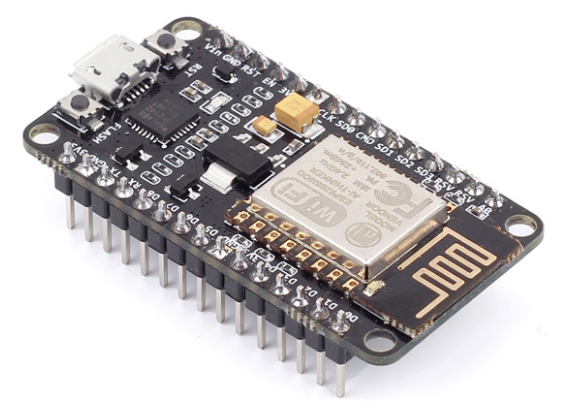
\includegraphics[scale=0.5]{mcu.PNG}
\caption{MCU ESP 8266}
\end{figure}


\subsection{MUX 74HC4051}
El 74HC4051 es un dispositivo útil que puede multiplexar (mux) o demultiplexar (demux) hasta 8 señales analógicas en una sola señal analógica.

Tiene un primo de 16 bits, el 74HC4067, que puede usarse para mux / demux hasta 16 señales.


\begin{figure}[H]
\centering
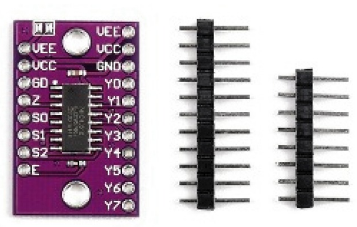
\includegraphics[scale=0.65]{mux.PNG}
\caption{MUX 74HC4051}
\end{figure}



\subsection{Sensor de calidad del Aire MQ135}



Este sensor se encarga de la detección de concentración de gas en diversos porcentajes, tal y como los son sus análogos MQ-3/4/5. La señal de salida que proporciona el MQ-135 es dual, de carácter analógico y digital. 

\begin{figure}[H]
\centering
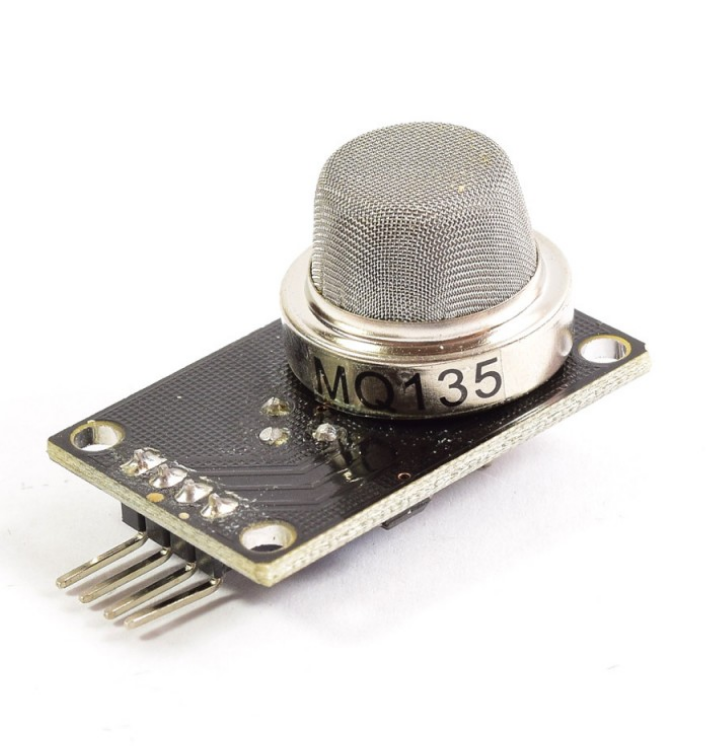
\includegraphics[scale=0.3]{mq35.PNG}
\caption{Sensor de calidad del aire MQ135}
\end{figure}


\begin{table}[H]
\centering
\begin{tabular}{|l|l|l|}
\hline
\multirow{4}{1cm}{MQ135} & Amoniaco & 100-300 \\ \cline{2-3}
& Alcohol & 10-300 \\ \cline{2-3}
& Benceno & 10-1000 \\ \cline{2-3}
& NOX, Humo y Dióxido de Carbono & No especificado \\ 
\cline{1-3}
\end{tabular}
\caption{Valores de Gases.}
\label{tabla:final}
\end{table}


\subsection{Sensor de Rayos UV GYML8511}
El sensor ML8511 UV (ultravioleta) funciona al emitir una señal analógica en relación con la cantidad de luz UV detectada. Esta ruptura puede ser muy útil para crear dispositivos que adviertan al usuario de quemaduras solares o detecten el índice UV en relación con las condiciones climáticas. \\


\begin{figure}[H]
\centering
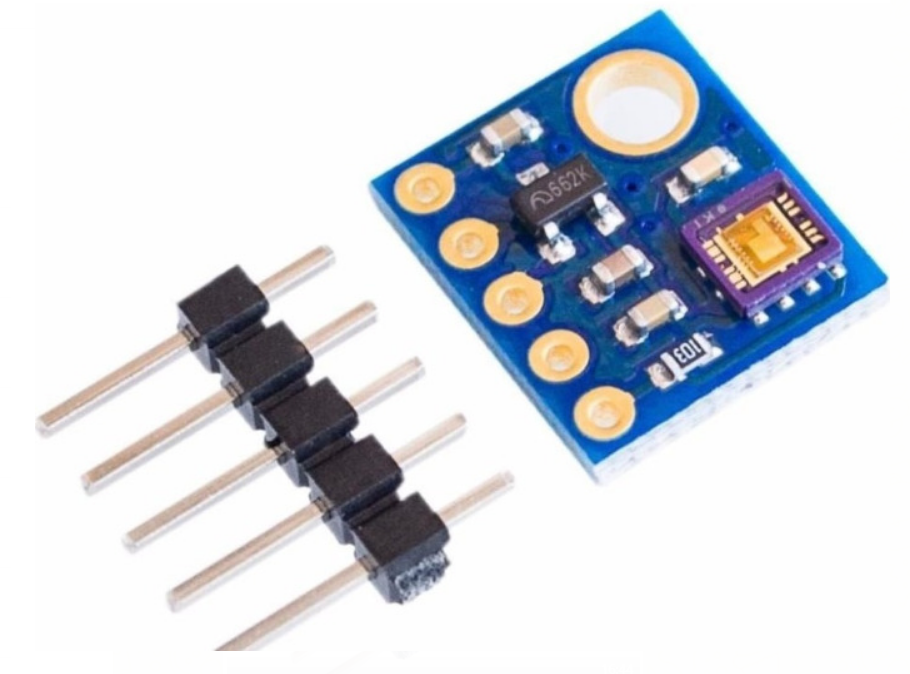
\includegraphics[scale=0.3]{Captura1.PNG}
\caption{Sensor de Rayos UV}
\end{figure}

\begin{figure}[H]
\centering
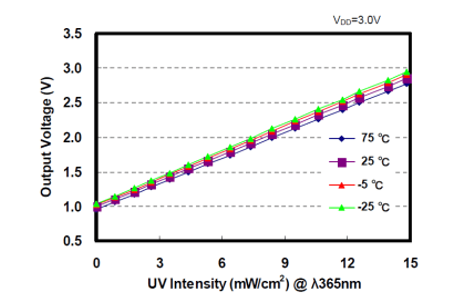
\includegraphics[scale=0.9]{indiceuv.PNG}
\caption{Comportamiento del Sensor}
\end{figure}

\begin{figure}[H]
\centering
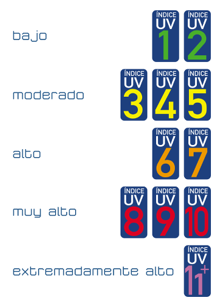
\includegraphics[scale=1]{uvindice.PNG}
\caption{Índice de rayos UV}
\end{figure}


\subsection{Sensor de C0 (monóxido de carbono) MQ7}
Está compuestos por un sensor electro-químico que varía su resistencia al estar en contacto con las sustancias.
Los sensores de gases son dispositivos con alta inercia, es decir, la respuesta necesita tiempos largos para estabilizarse tras un cambio de concentración de los gases medidos. 


\begin{figure}[H]
\centering
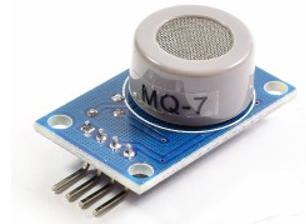
\includegraphics[scale=0.7]{Capturamq.PNG}
\caption{Sensor de CO MQ7}
\end{figure}


\begin{figure}[H]
\centering
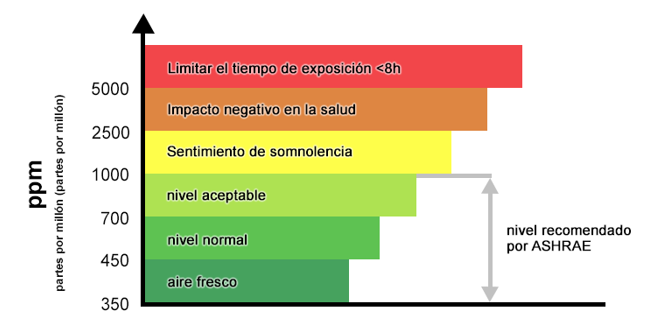
\includegraphics[scale=0.65]{escalamonoxido.PNG}
\caption{Escala de monóxido de Carbono}
\end{figure}
\subsubsection{Sensor de Temperatura y Humedad DHT11}
El DHT11 es un sensor digital de temperatura y humedad relativa de bajo costo y fácil uso. Integra un sensor capacitivo de humedad y un termistor para medir el aire circundante, y muestra los datos mediante una señal digital en el pin de datos (no posee salida analógica). 
\begin{figure}[H]
\centering
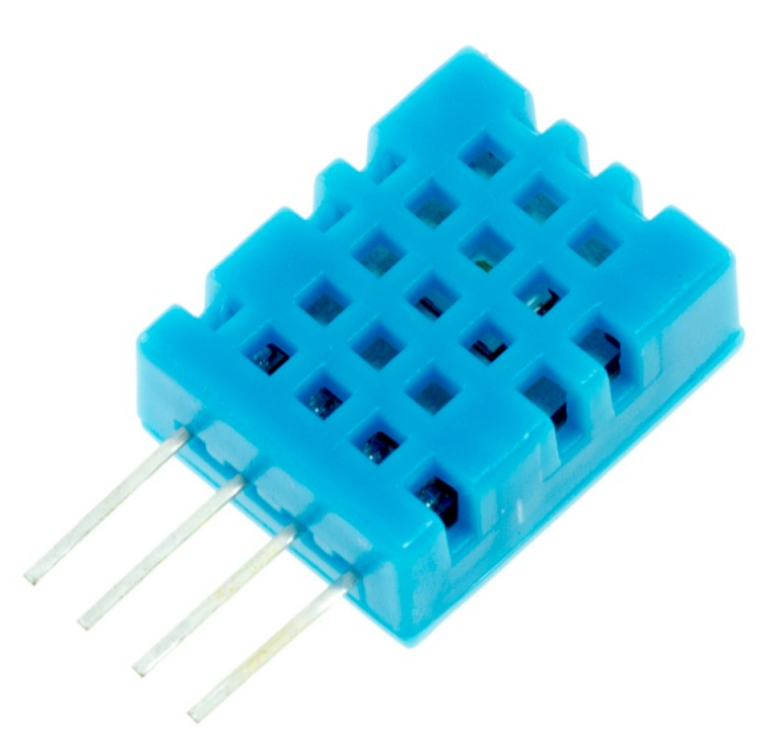
\includegraphics[scale=0.33]{dh.PNG}
\caption{Sensor de Temperatura y Humedad DHT11}
\end{figure}

\begin{figure}[H]
\centering
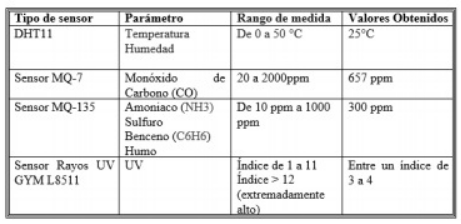
\includegraphics[scale=0.75]{tablita.PNG}
\caption{Escala de Sensores}
\end{figure}


\section{Desarrollo}
\subsection{Filtro  de suavisado Exponencial-Gaussiano}


\begin{figure}[H]
\centering
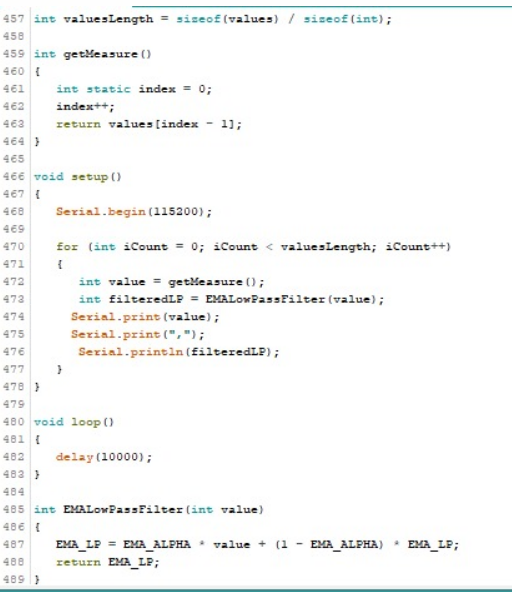
\includegraphics[scale=0.65]{codgauss.PNG}
\caption{Filtro de suavisado Exponencial-Gaussiano}
\end{figure}




\subsection{Filtro de suavisado Medio}

\begin{figure}[H]
\centering
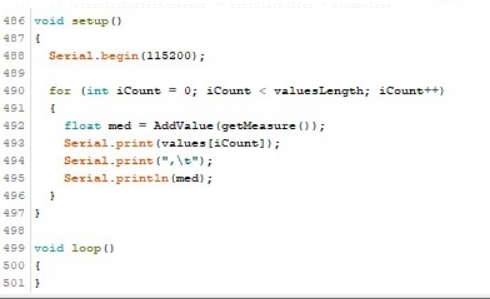
\includegraphics[scale=0.65]{codmedtwo.PNG}
\caption{Filtro de suavisado Medio}
\end{figure}


\begin{figure}[H]
\centering
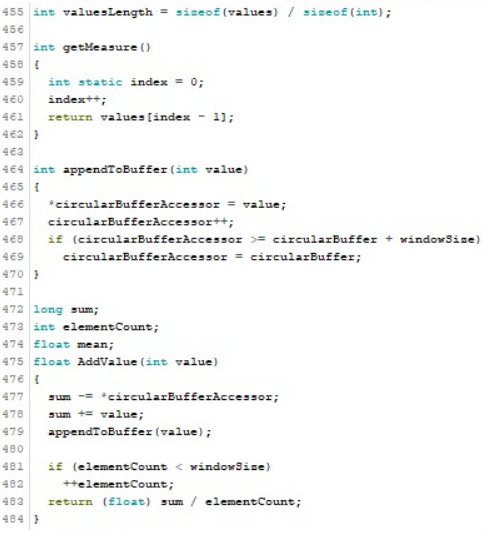
\includegraphics[scale=0.65]{codmedone.PNG}
\caption{Filtro de suavisado Medio}
\end{figure}


\subsection{Filtro de suavisado Mediano}
\begin{figure}[H]
\centering
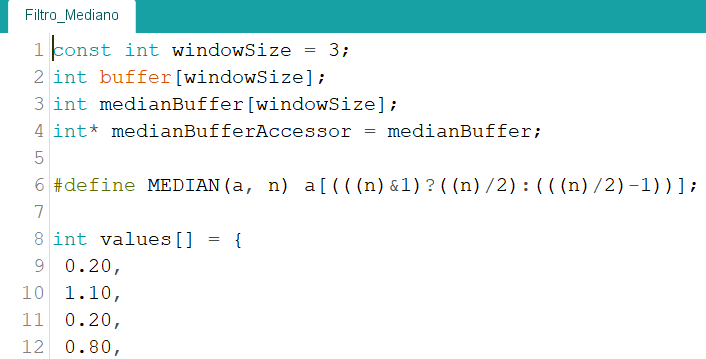
\includegraphics[scale=0.65]{coddianouno.PNG}
\caption{Filtro de Suavisado Mediano}
\end{figure}


\begin{figure}[H]
\centering
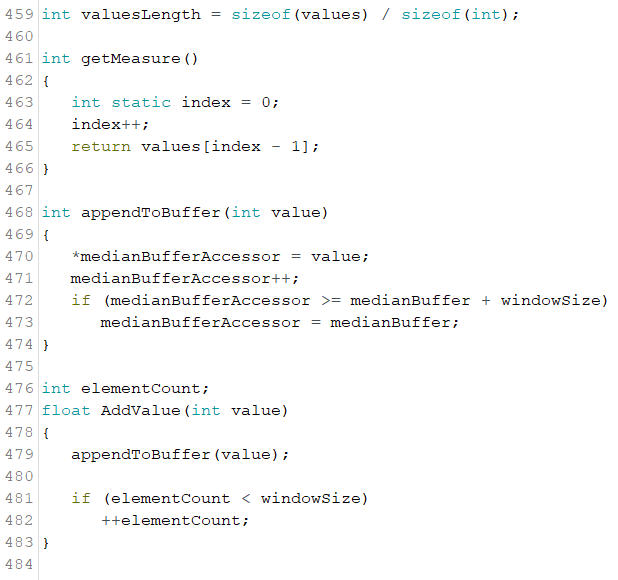
\includegraphics[scale=0.65]{coddianodos.PNG}
\caption{Filtro de Suavisado Mediano}
\end{figure}

\begin{figure}[H]
\centering
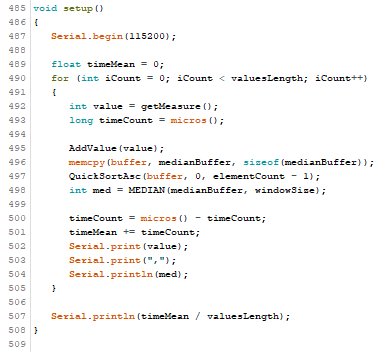
\includegraphics[scale=0.85]{codianotres.PNG}
\caption{Filtro de Suavisado Mediano}
\end{figure}

\begin{figure}[H]
\centering
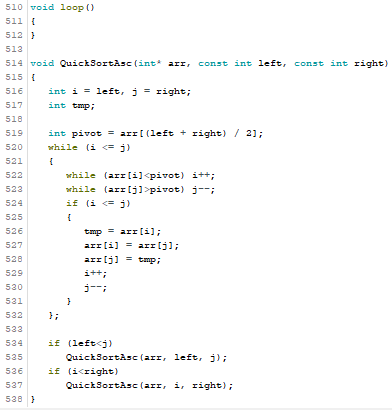
\includegraphics[scale=0.85]{coddianocuatro.PNG}
\caption{Filtro de Suavisado Mediano}
\end{figure}


\section{Análisis de Resultados}

Para la recolección de datos se ha tomado muestras de dos ambientes. El primer ambiente corresponde a un sector urbano y el segundo ambiente corresponde a un ambiente cercano al tubo de escape de un automóvil, se ha escogido estos dos ambientes con el fin de obtener variación en los datos y a la hora de filtrar las señales poder analizar los datos filtrados de una manera muy eficiente y de esta forma empezar a investigar en distintos ambientes que se pueda obtener acceso.\\
A continuación se muestran las gráficas obtenidas de cada filtro implementado en cada uno de los sensores (MCU,DHT11,MQ7,MQ135,UV) demostrando así los datos muestreados y filtrados, tomando en cuenta que la señal  muestreada está representada por el color azul y la señal filtrada está representada por el color rojo.
De acuerdo con los filtros analizados el mejor filtro de suavizado ha sido el filtro  Gaussiano nel cual  ha dado mejores valore MSE con respecto a las muestras que hemos aplicado este filtro. Por lo tanto este filtro es el más ideal para emplearlo en nuestro proyecto


\subsection{Análisis de Resultados con el Filtro Medio}

\subsubsection{Datos de Humedad-Sensor DHT11}


\begin{figure}[H]
\centering
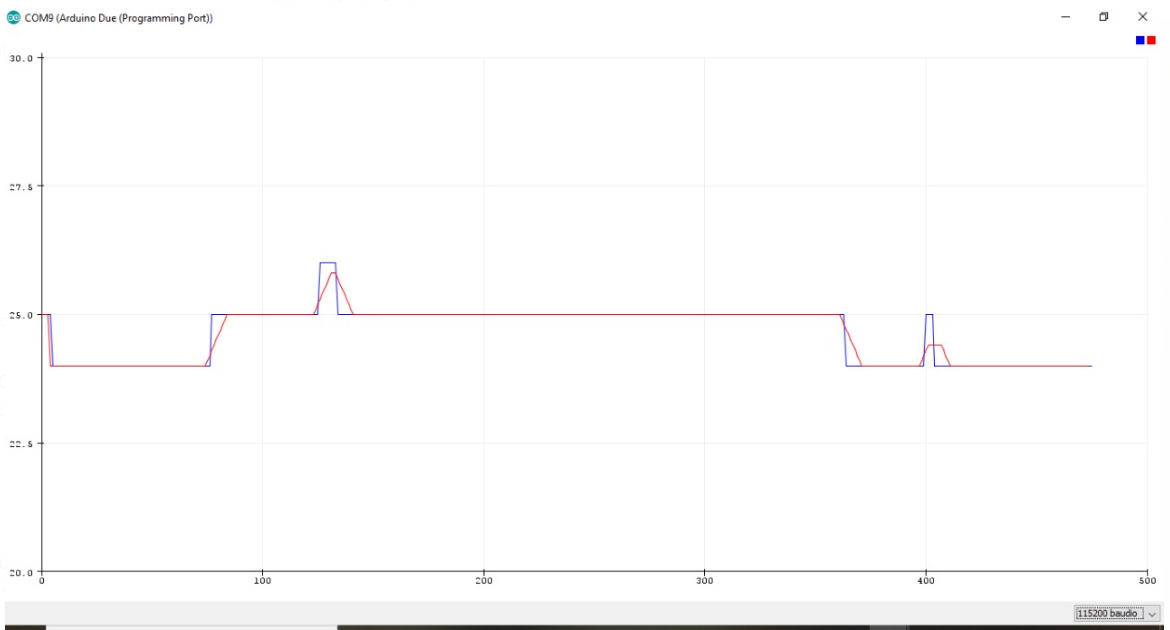
\includegraphics[scale=0.30]{dianohumedad.PNG}
\caption{Representación gráfica de Datos Muestreados y Filtrados}
\end{figure}


\subsubsection{Datos de Temperatura-Sensor DHT11}

\begin{figure}[H]
\centering
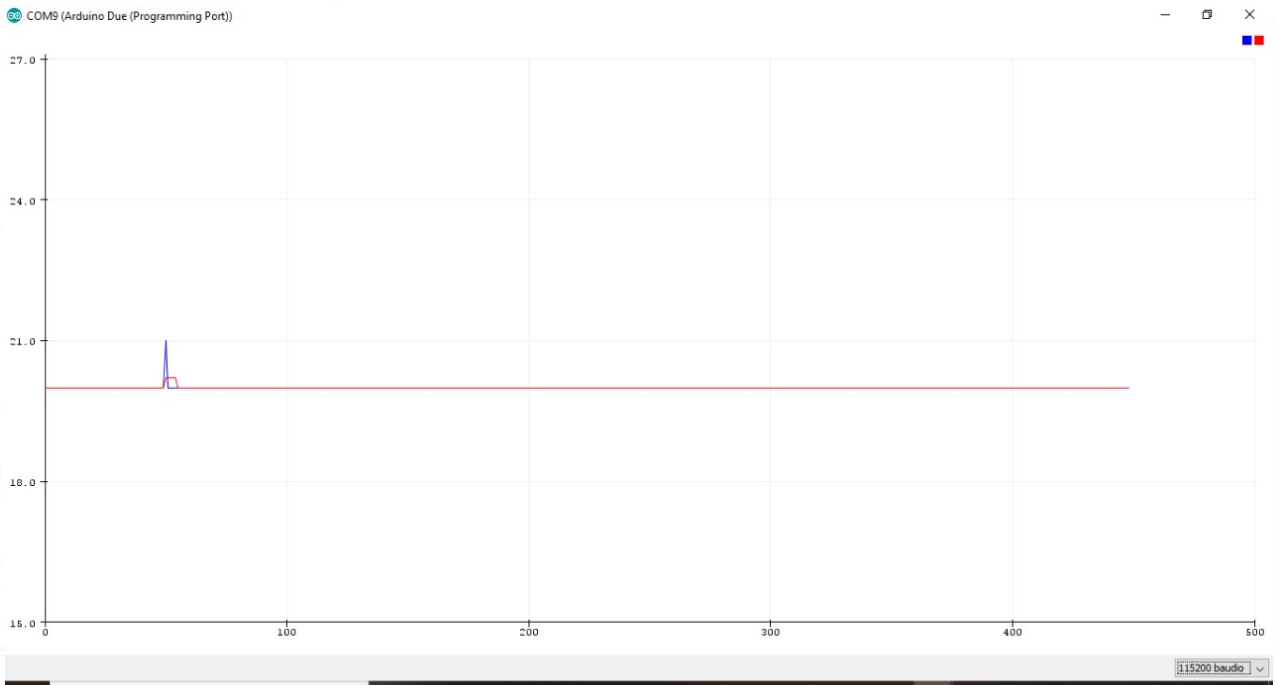
\includegraphics[scale=0.30]{dianotemperatura.PNG}
\caption{Representación gráfica de Datos Muestreados y Filtrados}
\end{figure}


\subsubsection{Datos de CO(Monóxido de Carbono)-Sensor MQ7}

\begin{figure}[H]
\centering
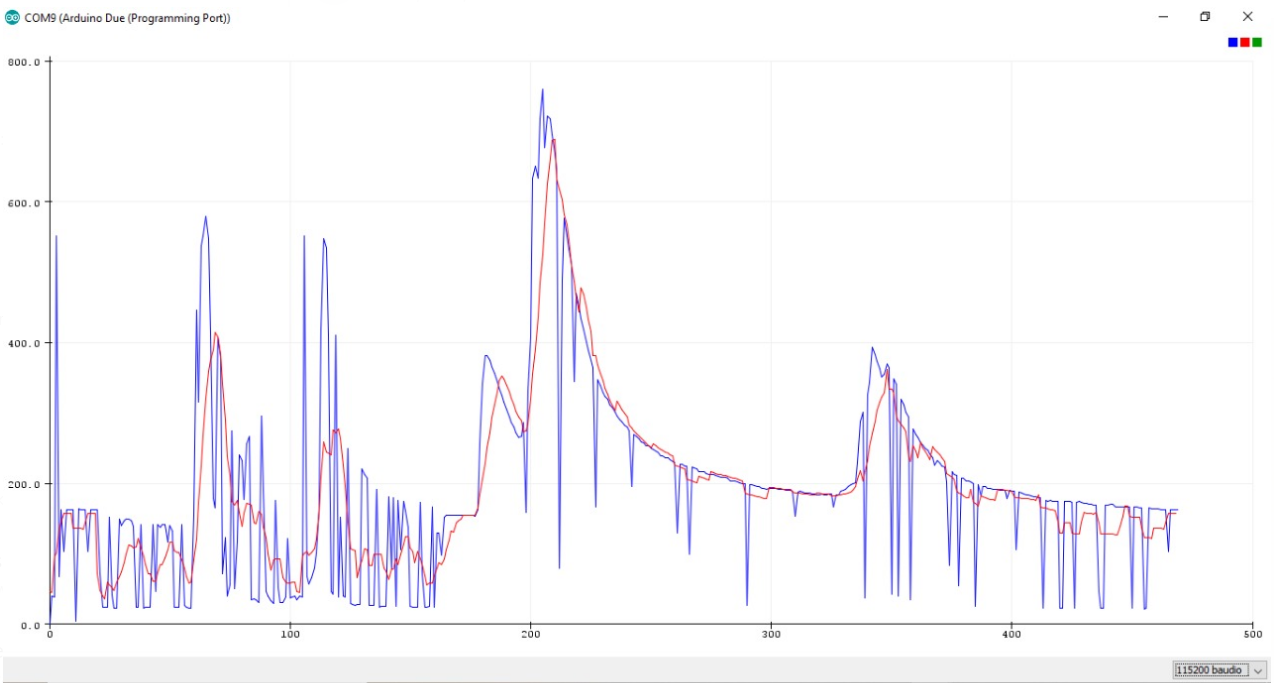
\includegraphics[scale=0.35]{dianomq7.PNG}
\caption{Representación gráfica de Datos Muestreados y Filtrados}
\end{figure}

\subsubsection{Datos de la calidad del aire -Sensor MQ135}

\begin{figure}[H]
\centering
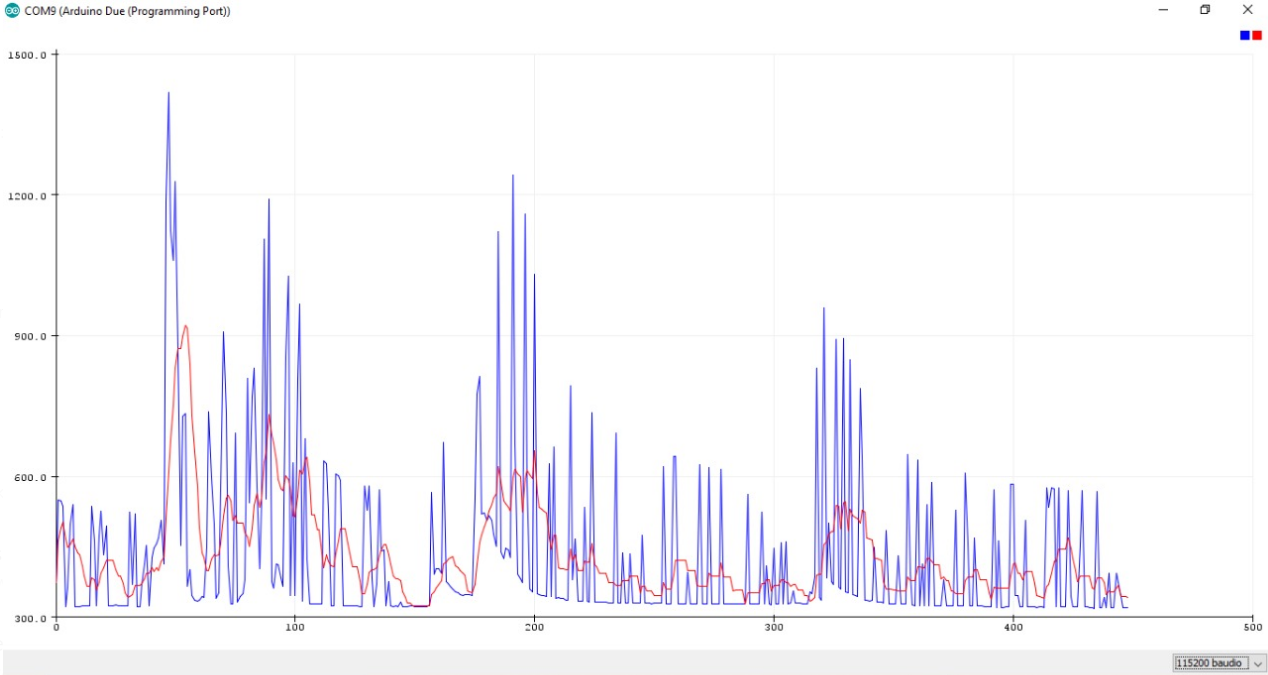
\includegraphics[scale=0.30]{dianomq135.PNG}
\caption{Representación gráfica de Datos Muestreados y Filtrados}
\end{figure}

\subsubsection{Datos de rayos UV-Sensor GYML8511}

\begin{figure}[H]
\centering
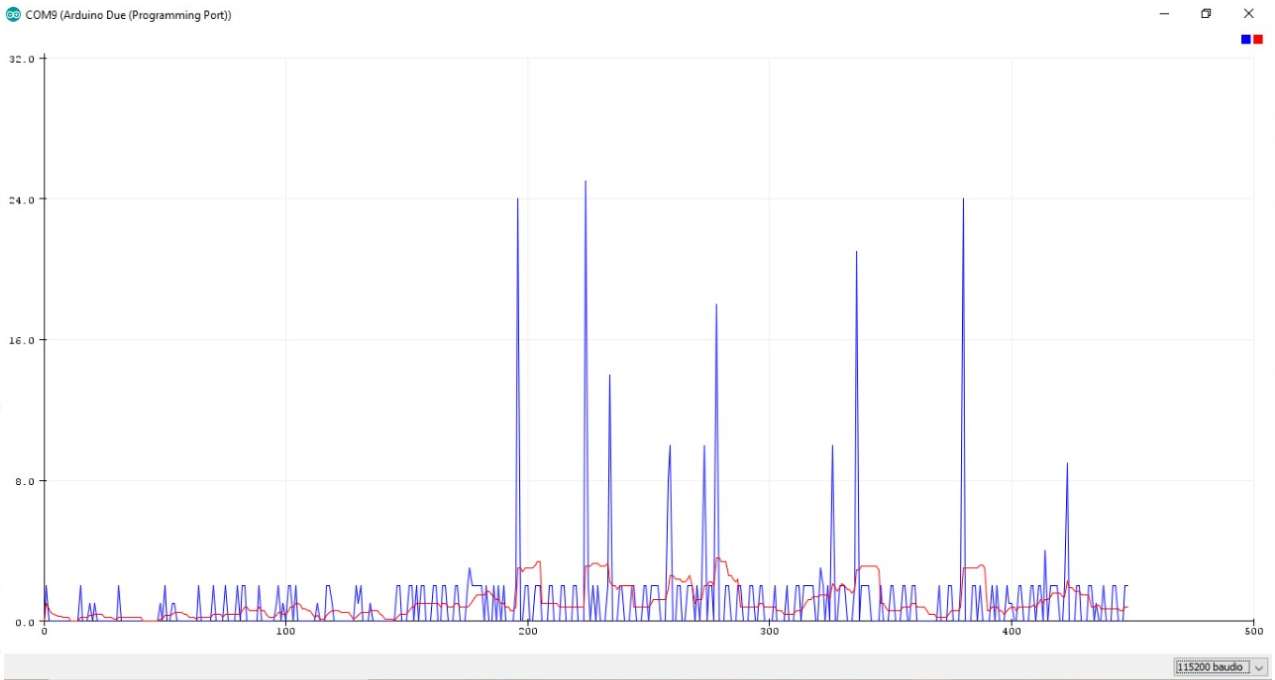
\includegraphics[scale=0.30]{dianouv.PNG}
\caption{Representación gráfica de Datos Muestreados y Filtrados}
\end{figure}

\subsection{Análisis de Resultados con el Filtro Exponencial-Gaussiano}

\subsubsection{Datos de Humedad-Sensor DHT11}

\begin{figure}[H]
\centering
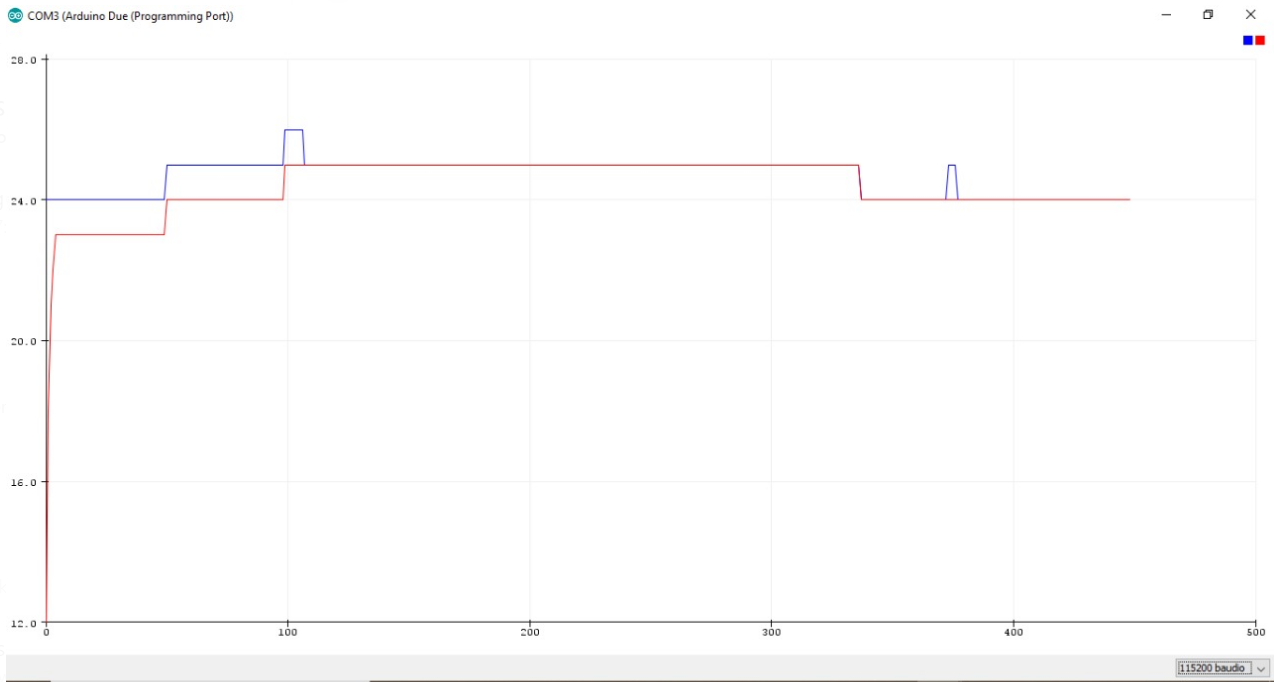
\includegraphics[scale=0.30]{medhumedad.PNG}
\caption{Representación gráfica de Datos Muestreados y Filtrados}
\end{figure}


\subsubsection{Datos de Temperatura-Sensor DHT11}


\begin{figure}[H]
\centering
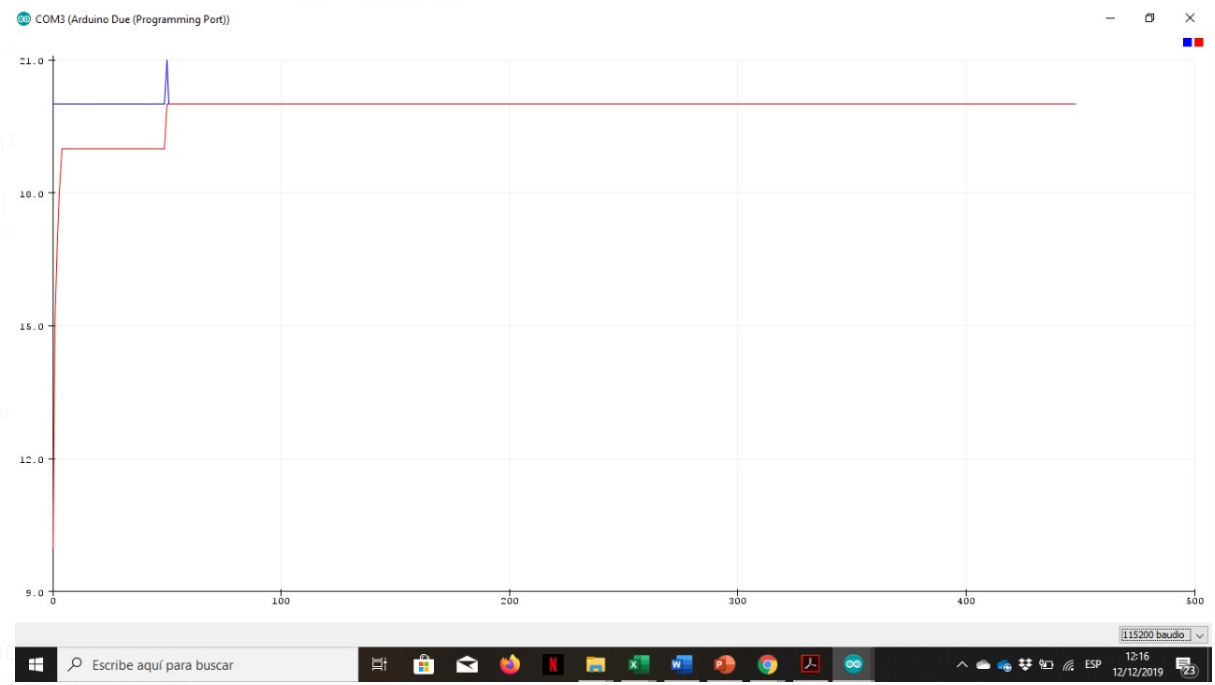
\includegraphics[scale=0.30]{medtemperatura.PNG}
\caption{Representación gráfica de Datos Muestreados y Filtrados}
\end{figure}


\subsubsection{Datos de CO(Monóxido de Carbono)-Sensor MQ7}

\begin{figure}[H]
\centering
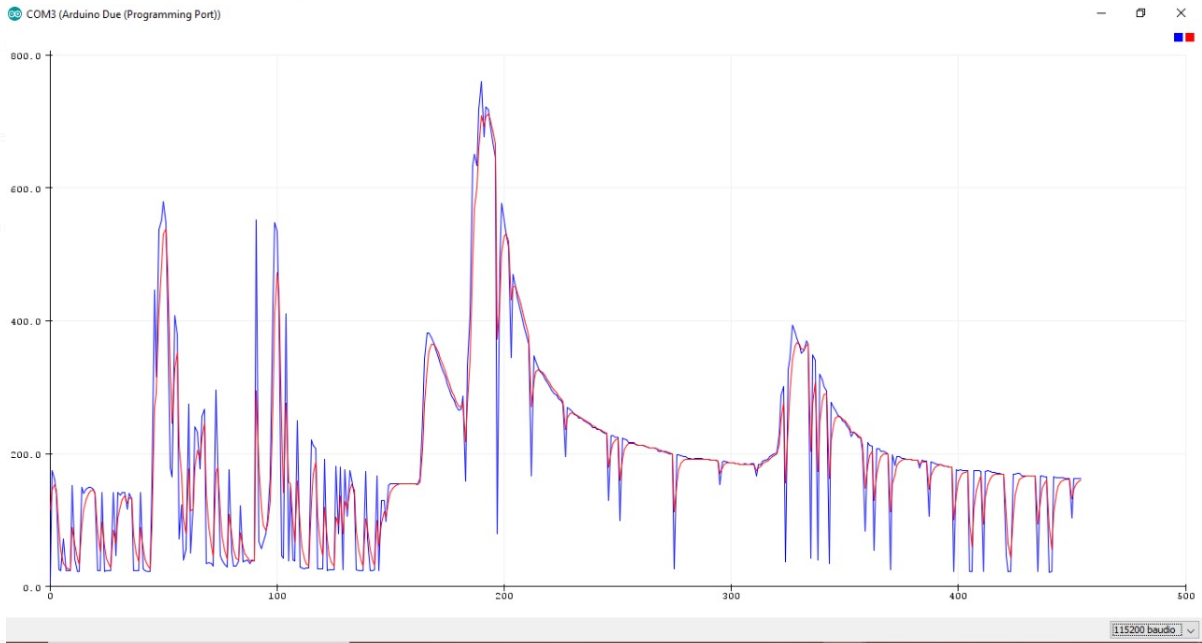
\includegraphics[scale=0.30]{medmq7.PNG}
\caption{Representación gráfica de Datos Muestreados y Filtrados}
\end{figure}


\subsubsection{Datos de la calidad del aire -Sensor MQ135}

\begin{figure}[H]
\centering
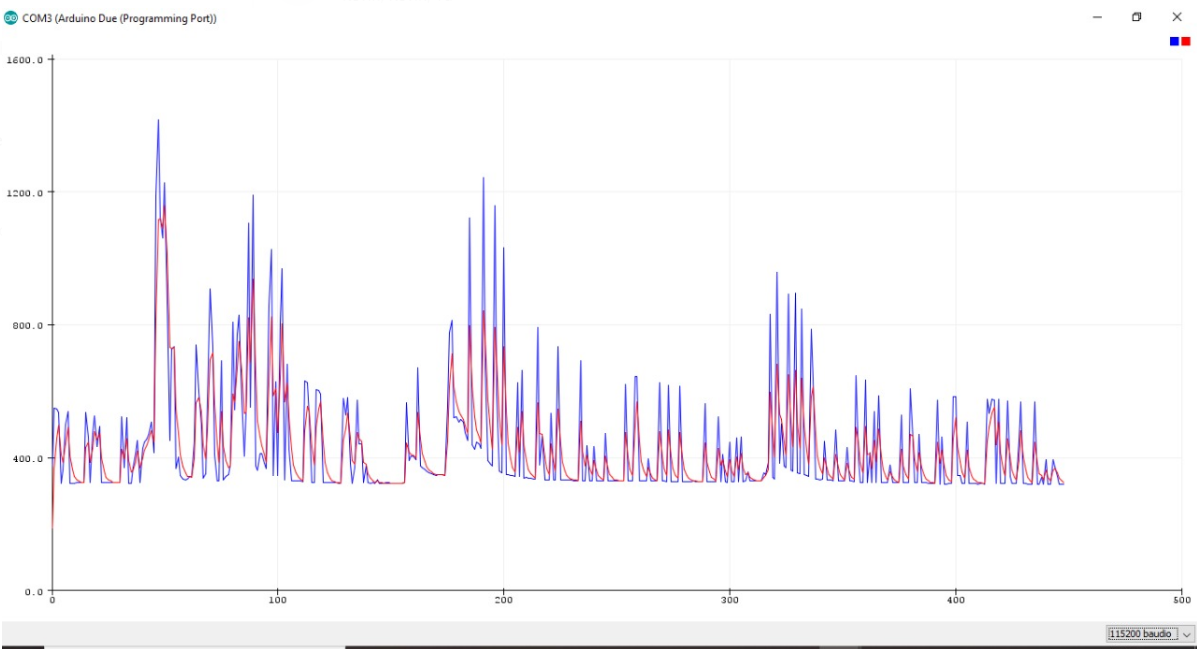
\includegraphics[scale=0.30]{medmq135.PNG}
\caption{Representación gráfica de Datos Muestreados y Filtrados}
\end{figure}

\subsubsection{Datos de rayos UV-Sensor GYML8511}

\begin{figure}[H]
\centering
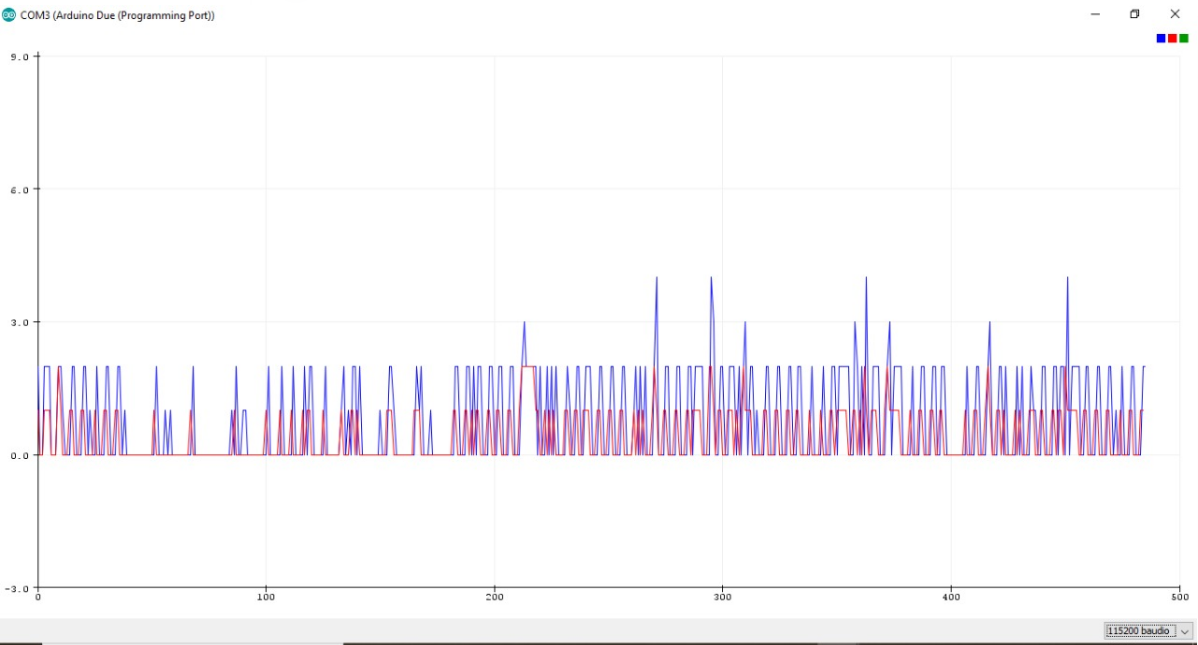
\includegraphics[scale=0.30]{meduv.PNG}
\caption{Representación gráfica de Datos Muestreados y Filtrados}
\end{figure}



\subsection{Análisis de Resultados con el Filtro Mediano}

\subsubsection{Datos de Humedad-Sensor DHT11}

\begin{figure}[H]
\centering
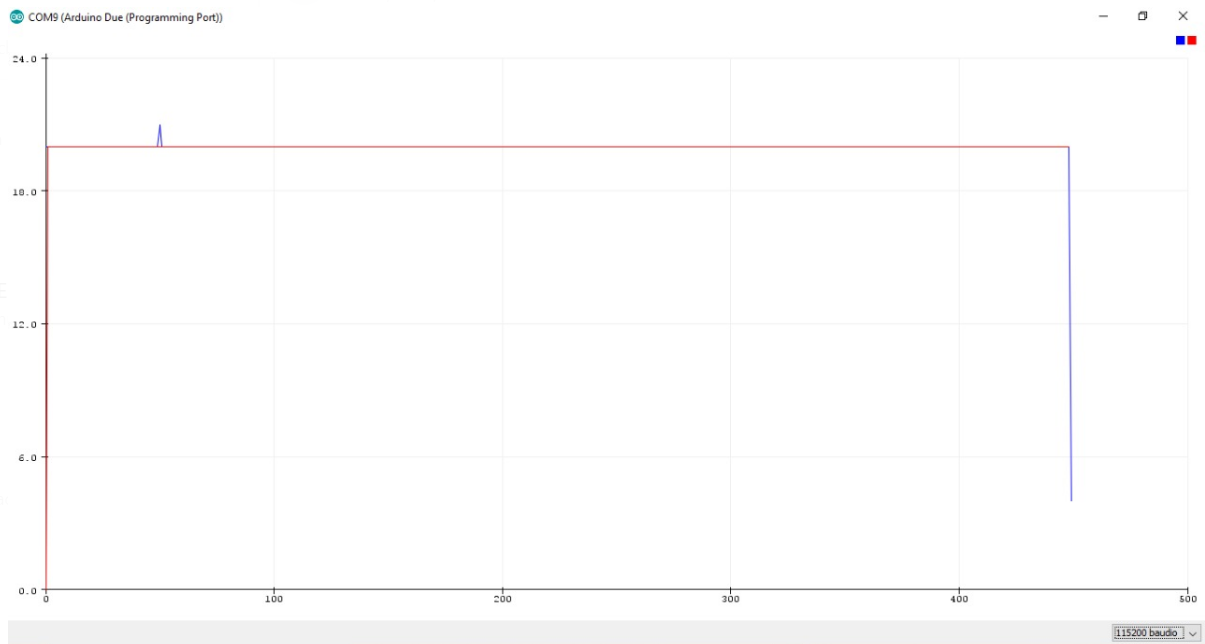
\includegraphics[scale=0.30]{gausstemperatura.PNG}
\caption{Representación gráfica de Datos Muestreados y Filtrado}
\end{figure}


\subsubsection{Datos de Temperatura-Sensor DHT11}

\begin{figure}[H]
\centering
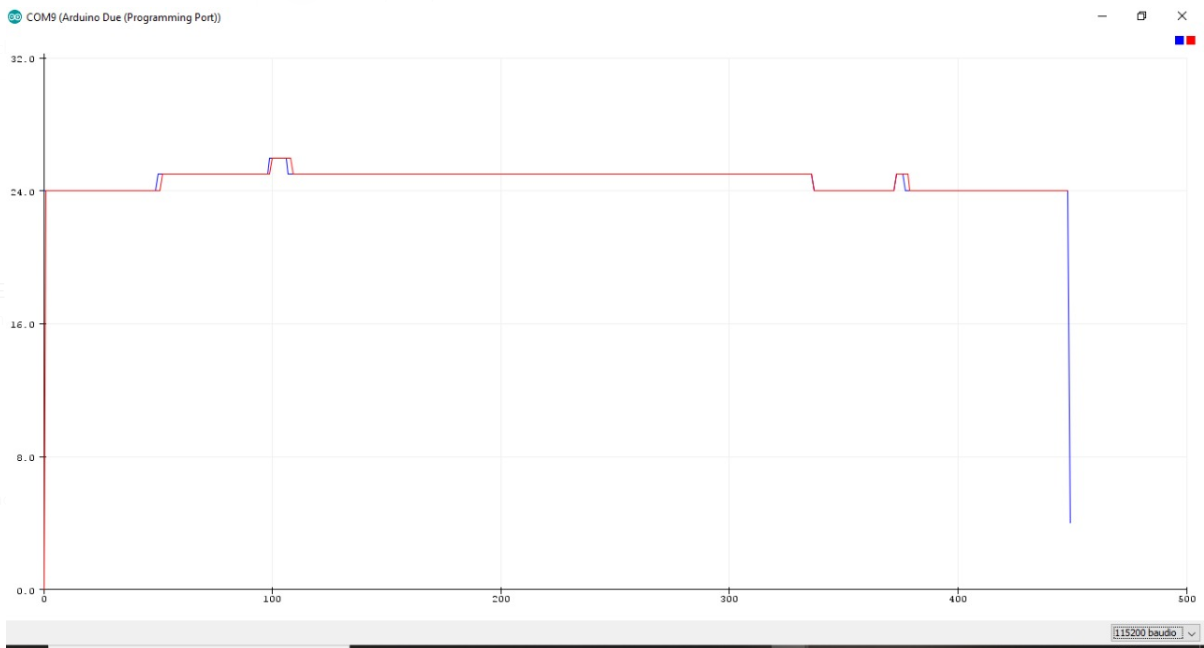
\includegraphics[scale=0.30]{gausshumedad.PNG}
\caption{Representación gráfica de Datos Muestreados y Filtrados}
\end{figure}


\subsubsection{Datos de CO(Monóxido de Carbono)-Sensor MQ7}

\begin{figure}[H]
\centering
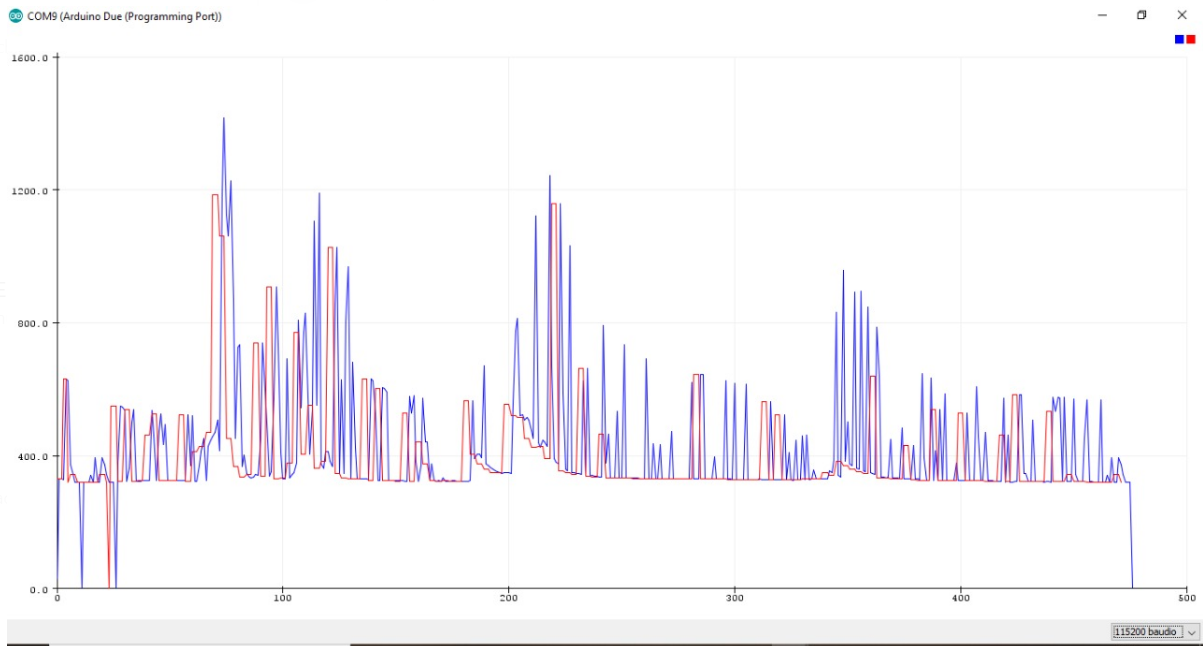
\includegraphics[scale=0.30]{gauusm7.PNG}
\caption{Representación gráfica de Datos Muestreados y Filtrados}
\end{figure}



\subsubsection{Datos de la calidad del aire -Sensor MQ135}
\begin{figure}[H]
\centering
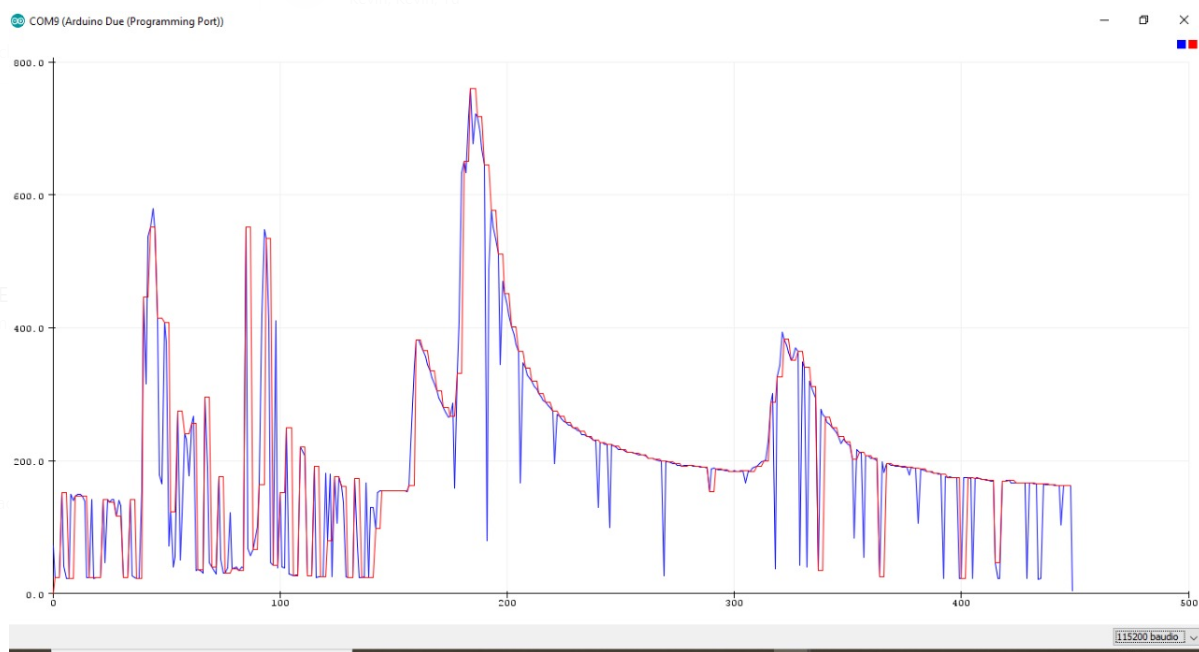
\includegraphics[scale=0.30]{gaussm135.PNG}
\caption{Representación gráfica de Datos Muestreados y Filtrados}
\end{figure}





\subsubsection{Datos de rayos UV-Sensor GYML8511}

\begin{figure}[H]
\centering
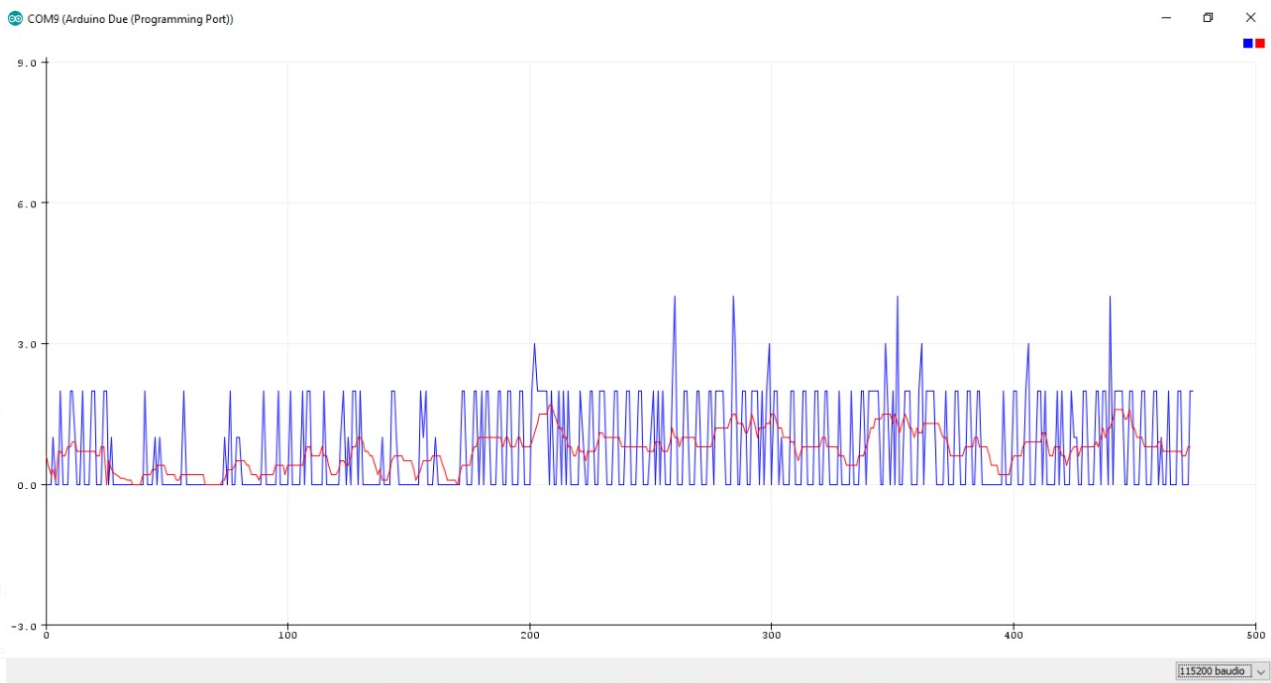
\includegraphics[scale=0.30]{gaussuv.PNG}
\caption{Representación gráfica de Datos Muestreados y Filtrados}
\end{figure}

\subsubsection{Tabla de Resultados}
\begin{figure}[H]
\centering
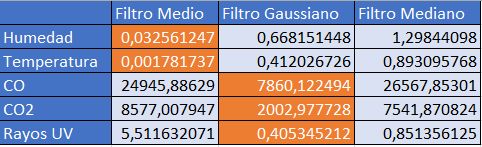
\includegraphics[scale=0.9]{result.PNG}
\caption{Tabla de Resultados}
\end{figure}
\begin{itemize}
\renewcommand{\labelitemi}{$-$}

\item Para el sensor de humedad el filtro que mejor suaviza la señal es el filtro Medio, ya que presenta una menor distancia entre los puntos que se están suavizando, por lo que se tiene un menor valor de MSE.\\
\\
\item Para el sensor de Temperatura el filtro que mejor suaviza la señal es el filtro Medio, ya que presenta una menor distancia entre los puntos que se están suavizando, por lo que se tiene un menor valor de MSE.\\
\item Para el sensor de CO el filtro que mejor suaviza la señal es el filtro Gaussiano, ya que presenta una menor distancia entre los puntos que se están suavizando, por lo que se tiene un menor valor de MSE .
\item Para el sensor de CO2 el filtro que mejor suaviza la señal es el filtro Gaussiano, ya que presenta una menor distancia entre los puntos que se están suavizando, por lo que se tiene un menor valor de MSE.
\item Para el sensor de Rayos UV el filtro que mejor suaviza la señal es el filtro Gaussiano, ya que presenta una menor distancia entre los puntos que se están suavizando, por lo que se tiene un menor valor de MSE.
\end{itemize}

\subsection{Diagrama de Bloques}

\begin{figure}[H]
\centering
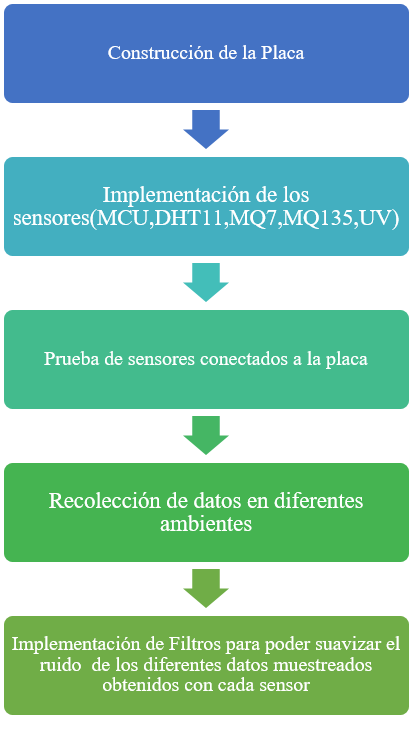
\includegraphics[scale=0.7]{bloquesDiagrama.PNG}
\caption{Diagrama de Bloques}
\end{figure}

\subsection{Flujograma de Actividades}
\begin{figure}[H]
\centering
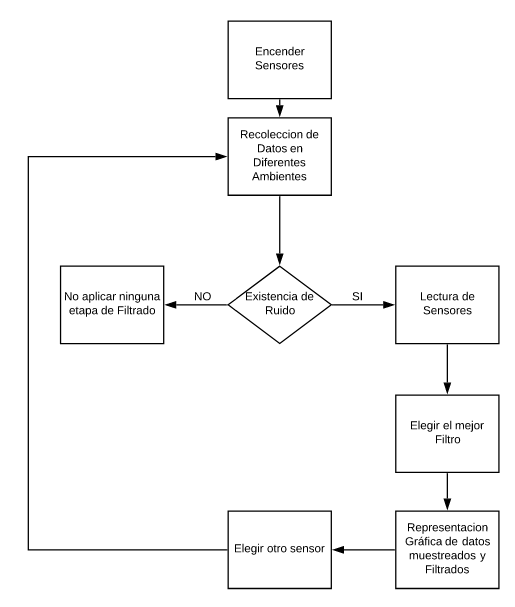
\includegraphics[scale=0.75]{flujo.PNG}
\caption{Flujograma de Actividaes}
\end{figure}

\subsection{Simulación en Fritzing}
\begin{figure}[H]
\centering
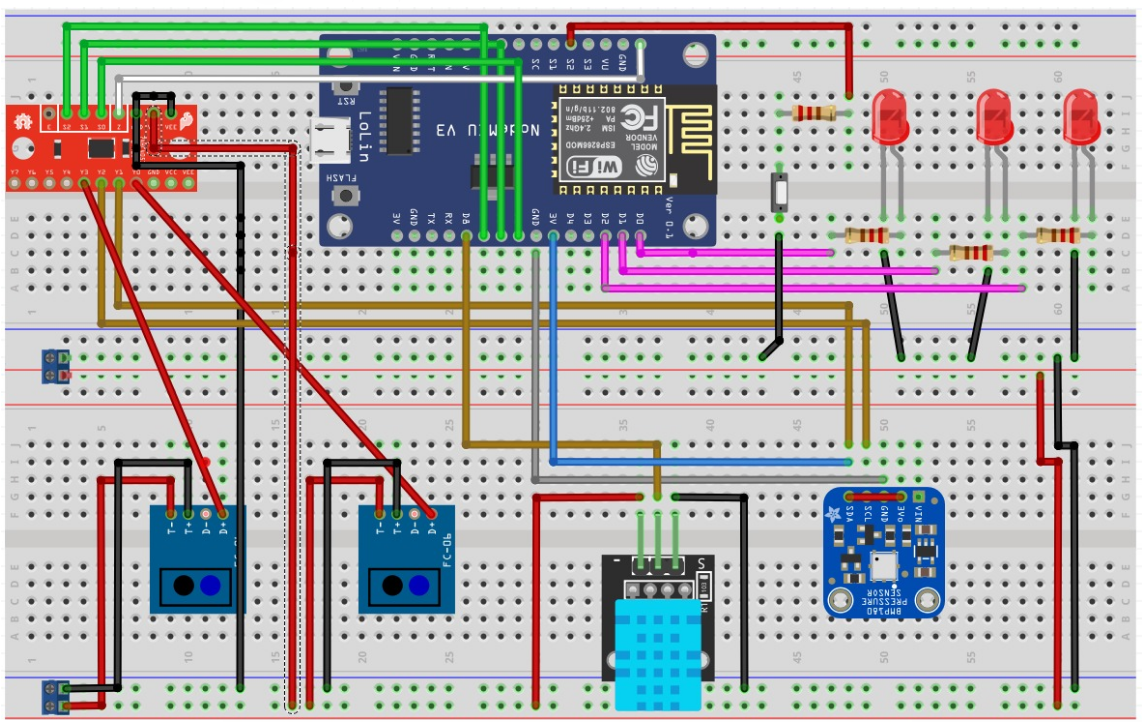
\includegraphics[scale=0.35]{frit.PNG}
\caption{Simulación en Fritzing}
\end{figure}

\subsection{Circuito Esquemático}
\begin{figure}[H]
\centering
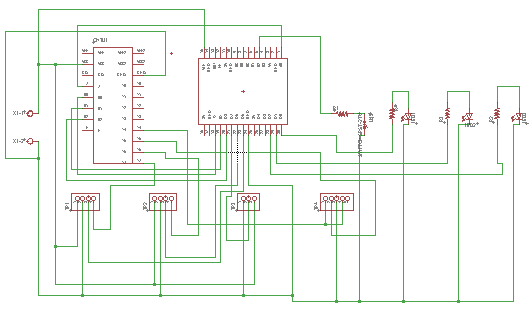
\includegraphics[scale=0.8]{esquematico.PNG}
\caption{Circuito Esquemático}
\end{figure}

\subsection{Diseño e Impresión del Circuito}
\begin{figure}[H]
\centering
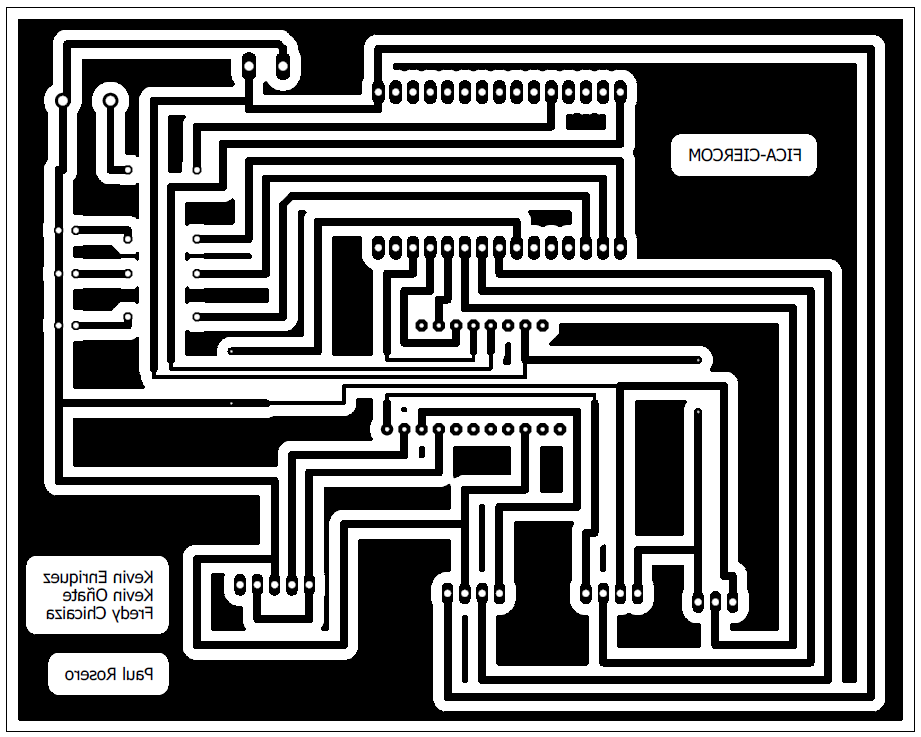
\includegraphics[scale=0.4]{placa.PNG}
\caption{Diseño e Impresión del Circuito}
\end{figure}


\subsection{Circuito implementado en Baquelita}

\begin{figure}[H]
\centering
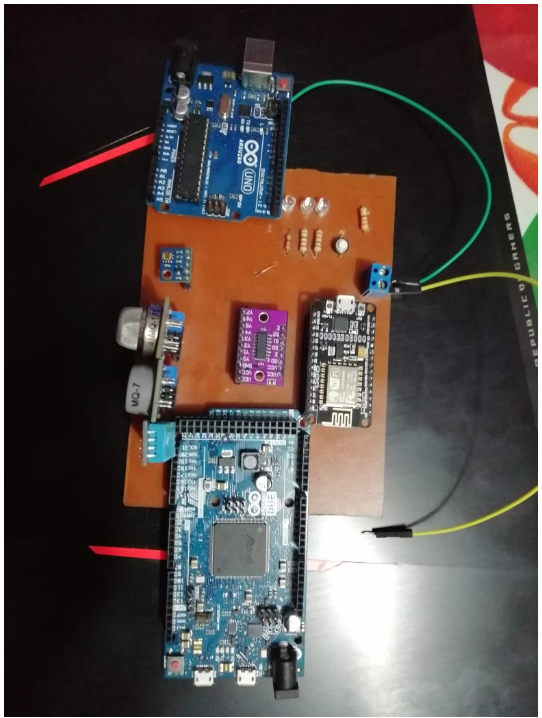
\includegraphics[scale=0.6]{dueyplaca.PNG}
\caption{Circuito implementado en Baquelita}
\end{figure}



\section{Conclusiones y Recomendaciones}

\textbf{Conclusiones:}
\begin{itemize}
\renewcommand{\labelitemi}{$-$}

\item El Filtro de suavizado Gaussiano nos ha dado mejores valore MSE con respecto a las muestras que hemos aplicado este filtro. Por lo tanto este filtro es el más ideal para emplearlo en nuestro proyecto.\\
\item Los sensores MQ, permiten detectar el nivel de presencia de ciertos gases toxico, por lo cual es necesario regularlos para detectar datos reales en el ambiente.\\

\item Para determinar el umbral de funcionamiento de cada uno de los sensores, es necesario revisar sus datasheets .\\
 
\item Dentro de la estructura del microprocesador ESP8266, el botón Flash permite guardar el programa dentro de la memoria del microprocesador.\\

\item Se ha  elegido como umbral mínimo 300 porque es difícil muestrear valores más bajos. Luego  se ha verificado si el valor de ppm es mayor que el de maxx, si es así, maxx  tomará ese valor.\\


 
\end{itemize}

\textbf{Recomendaciones:}
\begin{itemize}
\renewcommand{\labelitemi}{$*$}

\item Para obtener una mejor calibración se debe analizar las tablas de escala de referencia y valores, tanto del sensor de rayos UV como los sensores MQ.
 
\item Para no tener errores en la ejecución del código, se debe incluir las librerías que no estén actualizadas ya que las versiones anteriores ejecutan un buen proceso de recolección de datos referente al sensor.\\

\item Quemar los sensores de 11 a 48 horas ya que esto mejora su funcionamiento a la hora de recolectar los datos.\\



 
\end{itemize}

\section{Bibliografía}

[1] B. Fu, X. Xiong, and G. Sun, “An efficient mean filter algorithm,” in The 2011 IEEE/ICME International Conference on Complex Medical Engineering, May 2011, pp. 466–470.

[2] P. Shrivastava and U. P. Singh, “Noise removal using first order neighborhood mean filter,” in 2014 Conference on IT in Business, Industry and Government (CSIBIG), March 2014, pp. 1–6.

[3] P. K. Sinha and Q. H. Hong, “An improved median filter,” IEEE Transactions on Medical Imaging, vol. 9, no. 3, pp. 345–346, Sep 1990.

[4] N. C. Gallagher, “Median filters: a tutorial,” in 1988., IEEE International Symposium on Circuits and Systems, June 1988, pp. 1737–1744 vol.2.

[5] Z. Wang and D. Zhang, “Progressive switching median filter for the removal of impulse noise from highly corrupted images,” IEEE Transactions on Circuits and Systems II: Analog and Digital Signal Processing, vol. 46, no. 1, pp. 78–80, Jan 1999.

[6] T. Chen, K.-K. Ma, and L.-H. Chen, “Tri-state median filter for image denoising,” IEEE Transactions on Image Processing, vol. 8, no. 12, pp. 1834–1838, Dec 1999.





\begin{itemize}
\item Joan Ribas Lequerica.,(2015).Arduino para jóvenes y no tan jóvenes,España:ANAYA MULTIMEDIA.
\item Germán Tojeiro Calaza.,(2014).Taller de Arduino: un enfoque práctico para principiantes,Colombia:ALFAOMEGA.
\end{itemize}

\section{Anexos}


\begin{figure}[H]
\centering
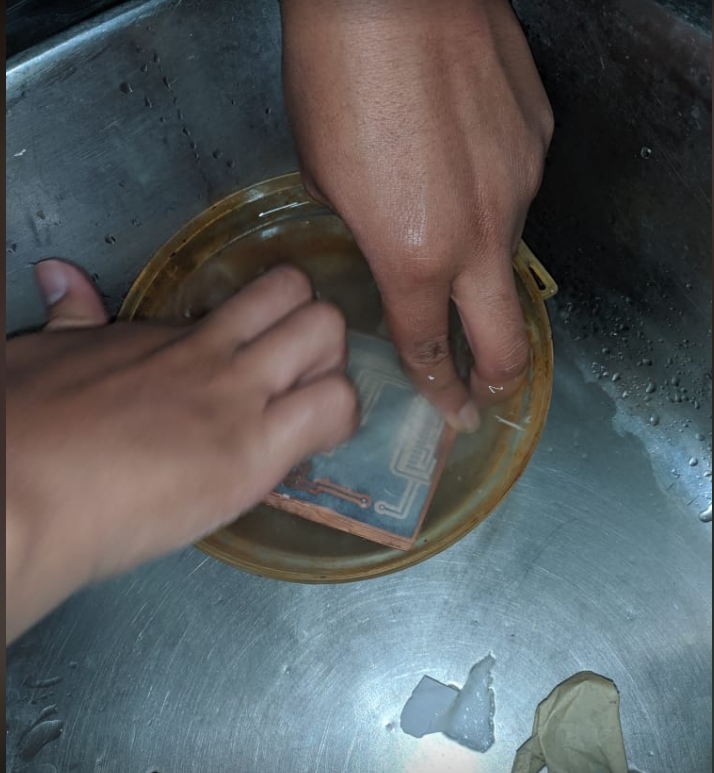
\includegraphics[scale=0.4]{anex.PNG}
\caption{Planchado del circuito en Baquelita}
\end{figure}
\begin{figure}[H]
\centering
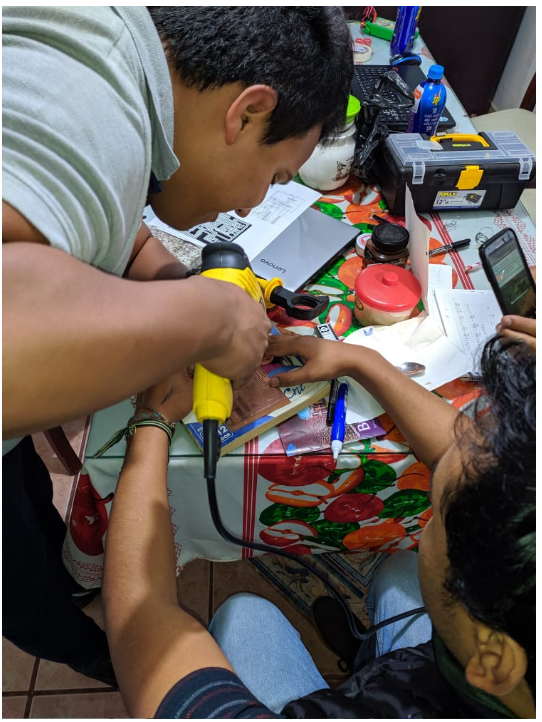
\includegraphics[scale=0.4]{anexito.PNG}
\caption{Perforación de Baquelita}
\end{figure}
\begin{figure}[H]
\centering
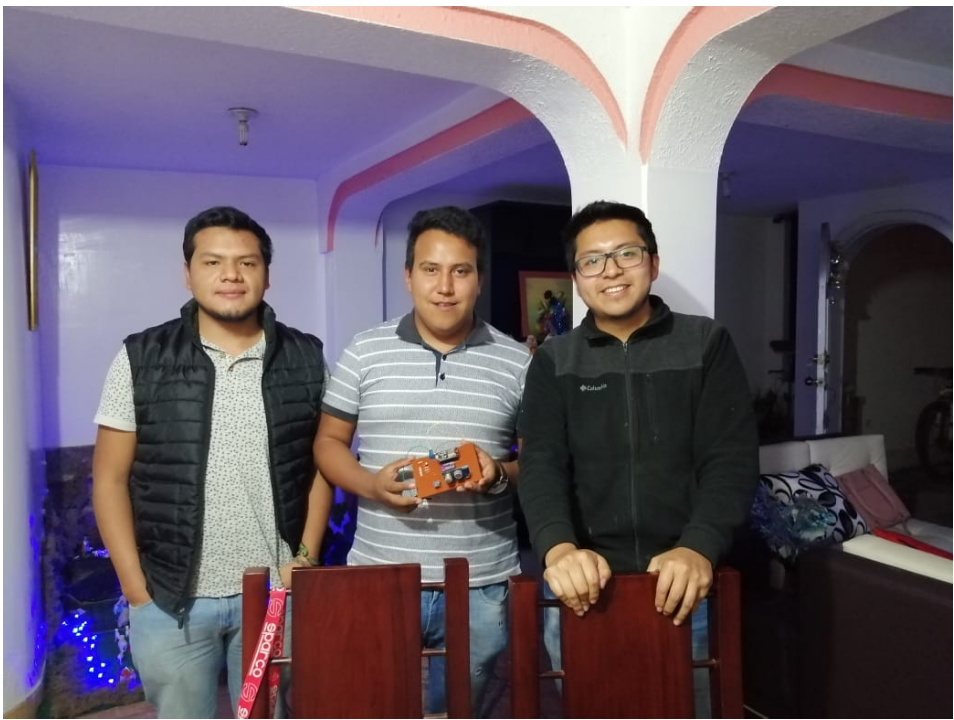
\includegraphics[scale=0.45]{equiptrab.PNG}
\caption{Equipo de Trabajo}
\end{figure}
\begin{figure}[H]
\centering
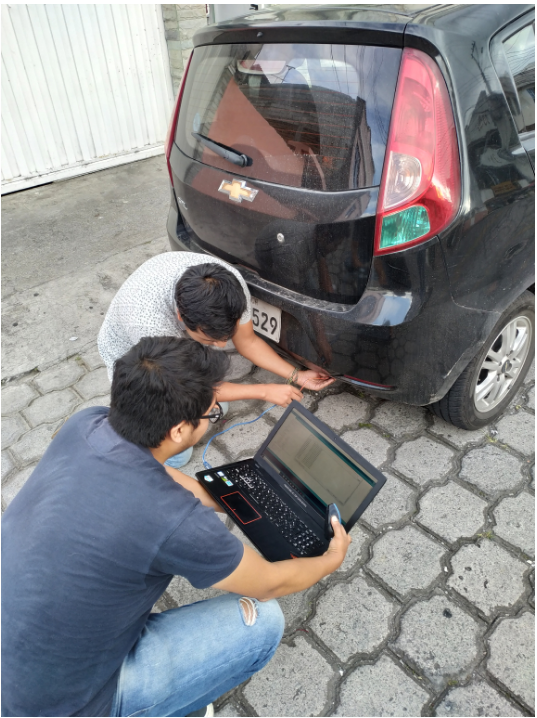
\includegraphics[scale=0.6]{datospruebas.PNG}
\caption{Recolección de datos en el tubo de escape de un automovil}
\end{figure}

\end{itemize}
\end{multicols}
\end{document}


\section{Enlaces Github}

https://github.com/Kevin-Onate/Sistemas-Embebidos/tree/master/Examen